%----------------------------------------------------------------------------
%----------------------------------------------------------------------------
\label{polarization damping}
%----------------------------------------------------------------------------
Suppose there exists an ensemble of molecules in which we can assign a classical dipole moment to each molecule. Let an incident beam of coherent linearly polarized light interact with each molecule through its dipole moment such that the coupling strength is proportional to $\hat{p} \cdot \hat{\varepsilon}$ where $\hat{p}$ is the direction of the dipole moment and $\hat{\varepsilon}$ the direction of the beam polarization. If the system is unprepared, i.e. we assume it is in thermodynamic equilibrium with its surroundings, the ``orientation polarization'' of the system will be completely incoherent.

Specifically, the normalized dipole vectors of the molecules will be uniformly distributed on the surface of the unit sphere and hence the projections of these vectors against the polarization axis of the incident light are also uniformly distributed. Thus, since the dipole interaction depends linearly on this projection, the distribution of coupling strengths in the ensemble will be uniformly distributed between zero and the maximum case (when the polarization and the dipole moment vectors point in the same direction).

%----------------------------------------------------------------------------
%----------------------------------------------------------------------------
%bb defines the bounding box for the pdf
%viewport defines the area of the pdf used
%in sidewaysfigure the last entry in bb moves the caption toward/away the pic
%in sidewaysfigure the second entry in bb moves the pic toward/away the caption
%----------------------------------------------------------------------------
\begin{figure}
\scalebox{0.8}[0.8]{
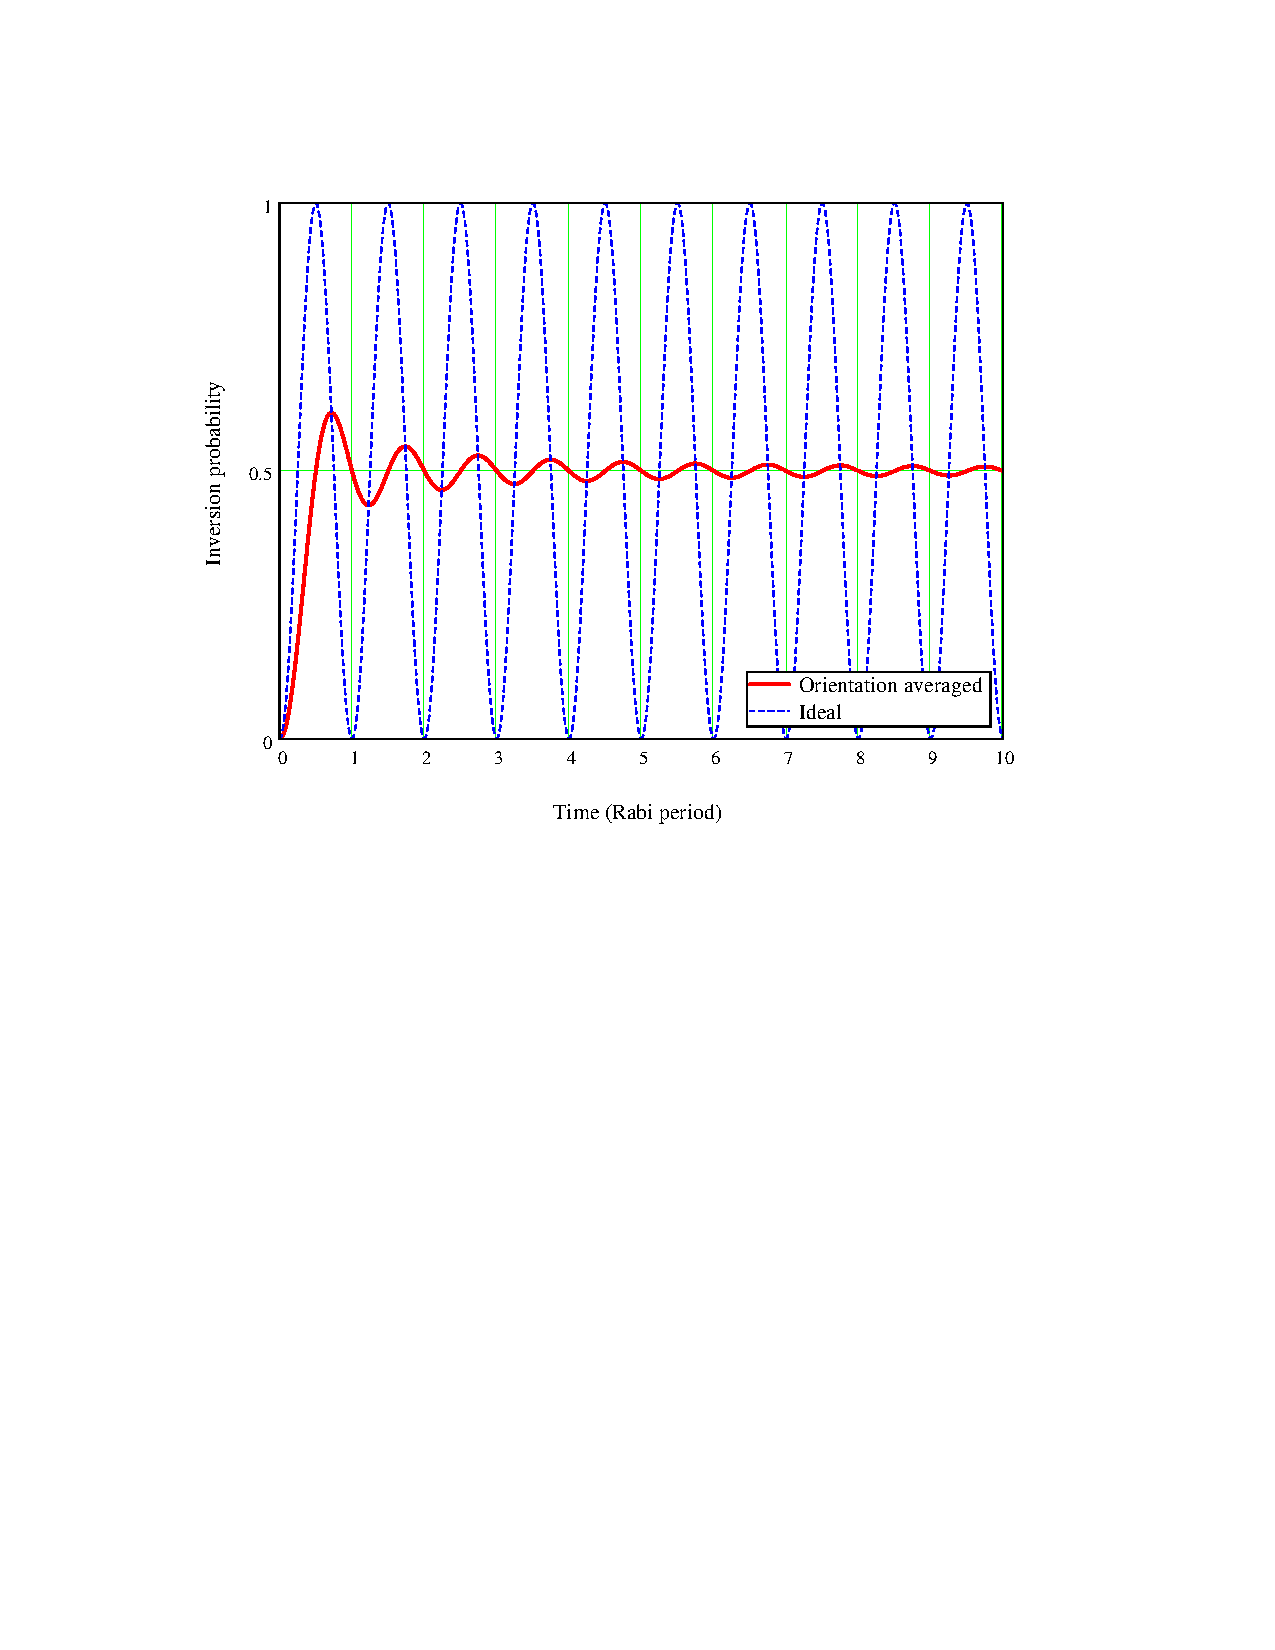
\includegraphics[bb=40 400 489 652]
{dynamics/dynamics.pdf}
}
\caption[Semi-classical behavior of a randomly oriented ensemble]{Semi--classical behavior of a randomly oriented ensemble. Equation \ref{2 level dynamics} is shown as the ``ideal'' behavior while the semi--classical result, Equation \ref{initial eom}, is called ``orientation averaged''.}
\label{dynamics}
\end{figure}
%----------------------------------------------------------------------------

%----------------------------------------------------------------------------
%bb defines the bounding box for the pdf
%viewport defines the area of the pdf used
%in sidewaysfigure the last entry in bb moves the caption toward/away the pic
%in sidewaysfigure the second entry in bb moves the pic toward/away the caption
%----------------------------------------------------------------------------
\begin{figure}
\scalebox{0.8}[0.8]{
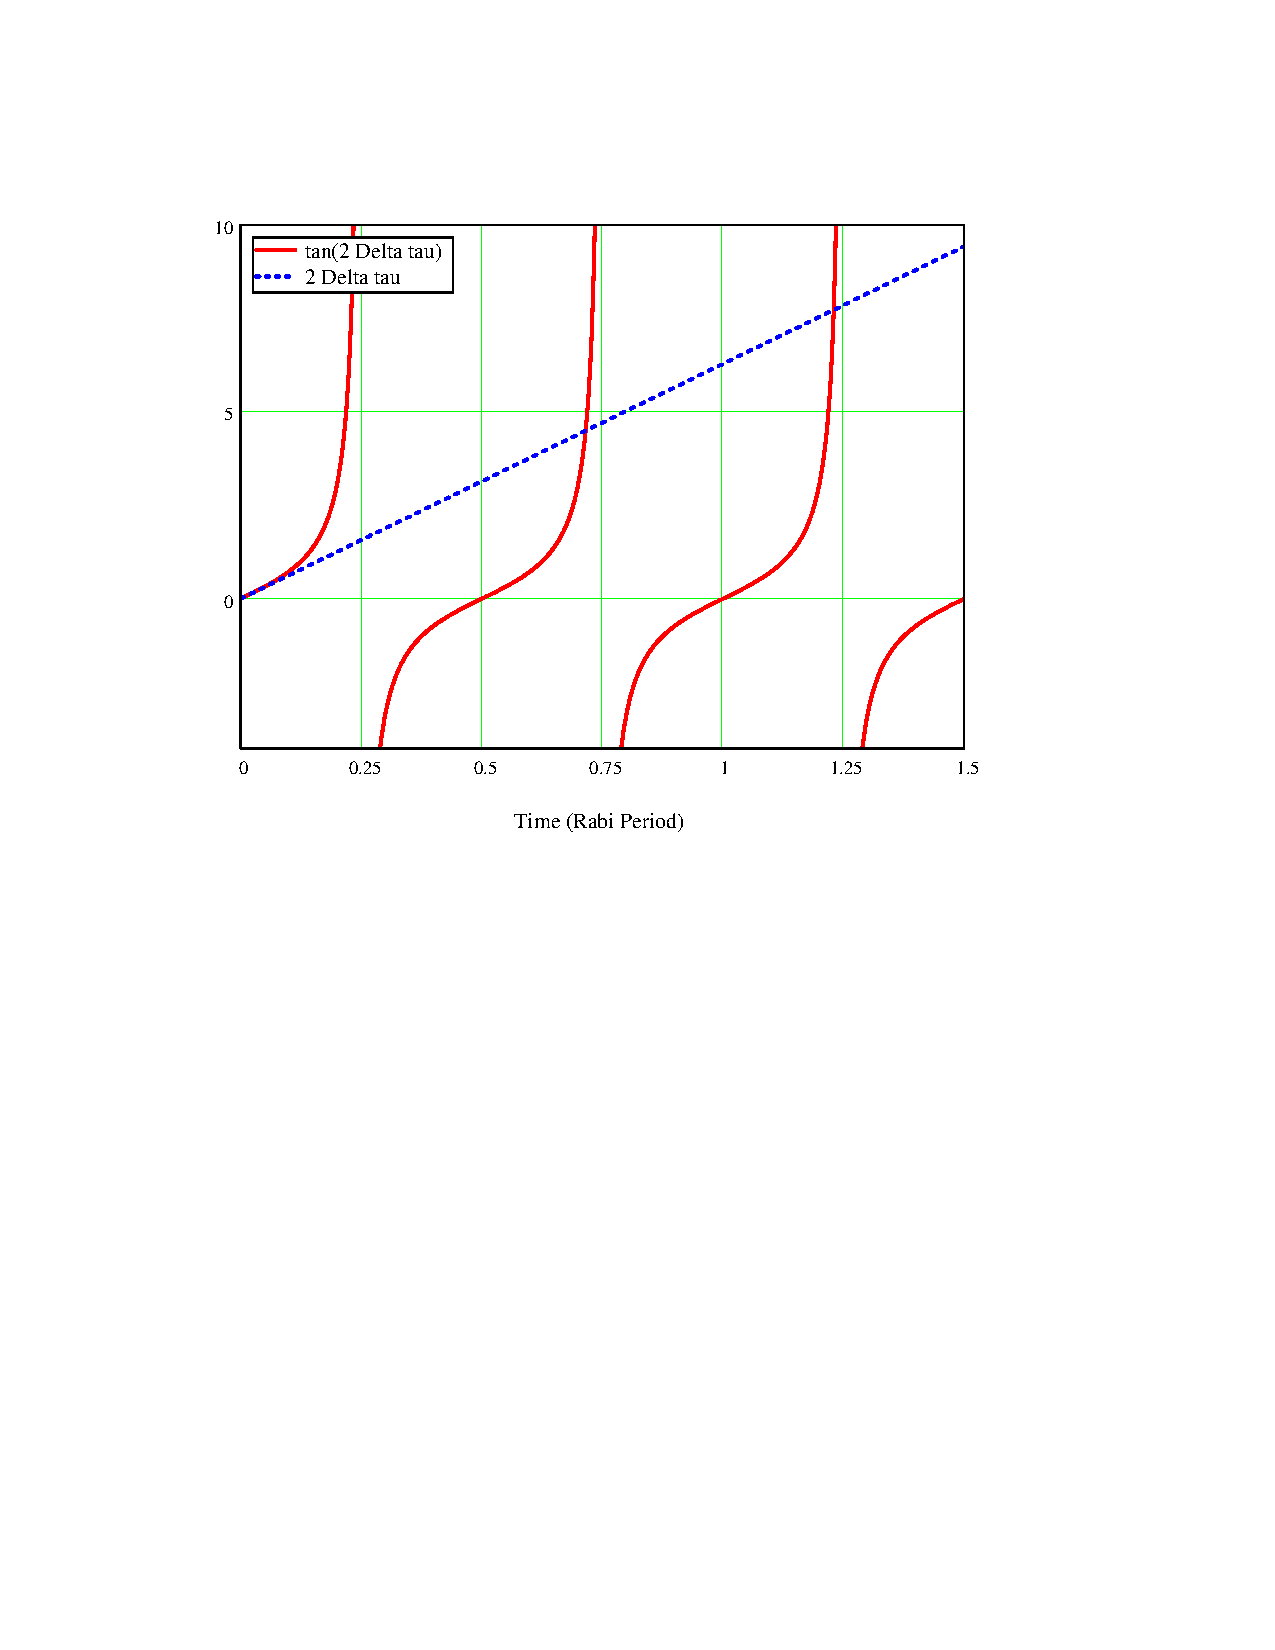
\includegraphics[bb=20 400 489 690]
{extremum/extremum.pdf}
}
\caption[Extremum of the orientation averaged dynamics]{Extremum of the averaged dynamics. The two intersections shown here represent the first absolute maxim and first local minim of the semi--classical behavior shown in Figure \ref{dynamics}. The first maximum has moved from 1/2 Rabi period to about 0.715148 Rabi period. The first minium, which ideally occurs at one Rabi period, has moved to about 1.229512 Rabi period.}
\label{extremum}
\end{figure}
%----------------------------------------------------------------------------

%----------------------------------------------------------------------------
Since the frequency of the Rabi oscillations depend linearly on the matrix element, the Rabi frequency is uniformly distributed in the ensemble. Now, for some molecule with a Rabi frequency reduced from the maximum by a factor $F\in[0,1]$, the probability of excitation at time $\tau$
%----------------------------------------------------------------------------
\begin{equation}
P_1(\tau)
=
\sin^2((F\Delta)\cdot\tau)
\end{equation}
%----------------------------------------------------------------------------
Thus, since the distribution is uniform, the average behavior of a (large) ensemble is
%----------------------------------------------------------------------------
\begin{equation}
P^{\prime}(\tau)
=
\int^{1}_{0}
\sin^2(F\Delta\tau)
dF
=
\frac{1}{2}
\left(
1-
\sinc{(2\Delta\tau)}
\right)
\label{initial eom}
\end{equation}
%----------------------------------------------------------------------------
or
%----------------------------------------------------------------------------
\begin{equation}
P^{\prime}(t)
=
\frac{1}{2}
\left(
1-
\sinc{(\Omega_R t)}
\right)
\label{initial eom normal}
\end{equation}
%----------------------------------------------------------------------------
where
%----------------------------------------------------------------------------
\begin{equation}
\sinc{(x)}
\equiv
\frac
{\sin{(x)}}
{x}.
\end{equation}
%----------------------------------------------------------------------------
See Figure \ref{dynamics} for a comparison between the ideal dynamics of a single molecule and the average behavior our thermal ensemble.

By examining the derivative of Equation \ref{initial eom} one finds that the extrema are located at the solutions to
%----------------------------------------------------------------------------
\begin{equation}
2 \Delta \tau
=
\tan{(2 \Delta \tau)}.
\end{equation}
%----------------------------------------------------------------------------
See Figure \ref{extremum} for a plot of the solution. The implications of these results are that more power will be required to induce the molecules to invert within a give time window (due to the forward shift of the maxima) and the resulting inversion probability will be reduced by a factor of $\sim0.6$. It can be shown that this is a worse case scenario (in terms of reduced modulation depth and forward shift of the maxima) when one compares this semi-classical behavior to the behavior resulting from a quantum mechanical treatment of the dipole approximation in the spherical harmonic basis set (personal communication, Pui K. Lam, June 2006).
%----------------------------------------------------------------------------
%----------------------------------------------------------------------------
